\chapter{Unsicherheitsfortpflanzung und Sensitivität}
\index{Unsicherheit}\index{Monte Carlo}\index{Sensitivität}
\section{Eingaben und zulässige Verteilungen}
Eine Verteilung benötigt eine begründete Quelle und eine SI-Einheit.
Ein zulässiges Materialintervall rechtfertigt allein noch keine Gleichverteilung;
ein Mittelwert allein keine Normalverteilung. Die Toolbox bietet diese
Verteilungen als explizite Nutzerannahmen an. Sie schätzt keine realen
Materialverteilungen aus fehlenden Messungen.

\texttt{Normal(mean, standard\_deviation)} verlangt eine positive endliche
Standardabweichung. Die Verteilung ist unbeschränkt: physikalisch ungültige
Materialziehungen werden nicht still gekappt. \texttt{Uniform(lower, upper)}
verlangt endliche streng geordnete Grenzen. Ein \texttt{UncertainParameter}
bindet Name, Modellpfad, Einheit, Verteilung und Begründung zusammen.
Das Ziel ist eine reelle skalare, im Kennwertvertrag definierte Größe.

\section{Sampling und Korrelation}
\texttt{SamplingPlan} verwendet NumPy PCG64 mit festem nichtnegativem Seed,
mindestens zwei gemeinsamen Parameterzeilen und einer dokumentierten
Samplingversion. Für unabhängige Normale gilt $X_i=\mu_i+\sigma_i Z_i$.
Unabhängige Gleichverteilungen werden über die Normalverteilungsfunktion
aus den standardnormalen Zeilen erzeugt.

Korrelation ist ausschließlich für gemeinsam normalverteilte Parameter
implementiert. Die Matrix $R$ muss endlich, symmetrisch, positiv semidefinit
und auf der Diagonale 1 sein; die Rundungstoleranz ist $10^{-12}$.
Die Eigenzerlegung bildet eine Quadratwurzel, sodass auch singuläre zulässige
Matrizen möglich sind. Für Normalparameter lautet die Kovarianz
\begin{equation}
 \operatorname{Cov}(X_i,X_j)=\sigma_i\sigma_jR_{ij}.
\end{equation}
Abhängige Gleichverteilungen und gemischte korrelierte Familien werden
abgelehnt. Es gibt keinen impliziten Copula-Vertrag. Die Zeilen sind gegen
Änderung geschützt; Spezifikation, Softwareversionen und Hashes halten die
Herkunft fest. Ein Seed allein ersetzt diese Informationen nicht.

\section{Statistik und lokale Ableitungen}
Für $n$ erfolgreiche Werte $f_k$ berechnet der Workflow
\begin{equation}
 \bar f=\frac1n\sum_k f_k,\qquad
 s^2=\frac1{n-1}\sum_k(f_k-\bar f)^2.
\end{equation}
Die Varianz ist die unverzerrte Stichprobenvarianz. Quantile nutzen lineare
Interpolation mit dokumentierten Wahrscheinlichkeiten. Präfixe der Länge
$2,4,8,\ldots,n$ zeigen den Verlauf der Schätzung. Sie sind weder ein
automatisches Abbruchkriterium noch ein Konfidenzband.

Die lokale Sensitivität am ausdrücklich gewählten Zentrum lautet
\begin{equation}
 g_i\approx\frac{F(\mathbf x+h_i\mathbf e_i)-F(\mathbf x-h_i\mathbf e_i)}{2h_i}.
\end{equation}
Sie benötigt $2p$ Auswertungen und endliche positive Schritte in der jeweiligen
Parametereinheit. Ihre Einheit ist Zieleinheit pro Parametereinheit. Bei einem
nichtlinearen Fall müssen Schrittverkleinerung und Solverrauschen untersucht
werden. Diese lokalen Ableitungen sind keine globalen Sobol-Indizes und keine
Aussage zur Wichtigkeit über eine ganze Verteilung.

\section{Analytischer korrelierter Referenzfall}
Der synthetische Fall hat dimensionslose Eingaben
$X\sim\mathcal N(1,2^2)$, $Y\sim\mathcal N(-2,3^2)$, $\rho=0.5$ und
$F=4+2X-Y$ mit Koeffizienten in K. Unabhängig vom Sampling folgt
\begin{align}
 \mathbb E[F]&=4+2\cdot1-(-2)=8\ \mathrm K,\\
 \operatorname{Var}(F)&=4\cdot4+9-4\cdot(0.5\cdot2\cdot3)
 =13\ \mathrm K^2,\\
 \nabla F&=(2,-1)\ \mathrm K.
\end{align}
Die vorab bestehende Testregel akzeptiert beim Mittelwert sechs analytische
Standardfehler $6\sqrt{13/n}$ und bei der Varianz
$6\cdot13\sqrt{2/(n-1)}$. Diese breiten stochastischen Testschranken sichern
die Implementierung; sie sind keine experimentellen Akzeptanzgrenzen.
Es werden 100\,000 Zeilen mit Seed 641 erzeugt. Die Tabelle und Abbildung
entstehen aus dem gespeicherten Ergebnis, nicht aus von Hand gerundeten Kopien.

\begin{table}[htbp]\centering
% Generated; review sources before regenerating.
\begin{tabular}{lrr}\toprule Größe & Analytisch & Stichprobe\\\midrule
Mittelwert / K & 8 & 8.00739218\\
Varianz / K$^2$ & 13 & 13.00581914\\
Quantil 0.025 / K & --- & 0.95832486\\
Quantil 0.5 / K & --- & 8.01277839\\
Quantil 0.975 / K & --- & 15.07179933\\
\bottomrule\end{tabular}

\caption{Reproduzierter synthetischer Referenzfall, $n=100\,000$, Seed 641.
Die Quantile sind Stichprobenwerte; keine Messdaten.}
\end{table}

\begin{figure}[htbp]\centering
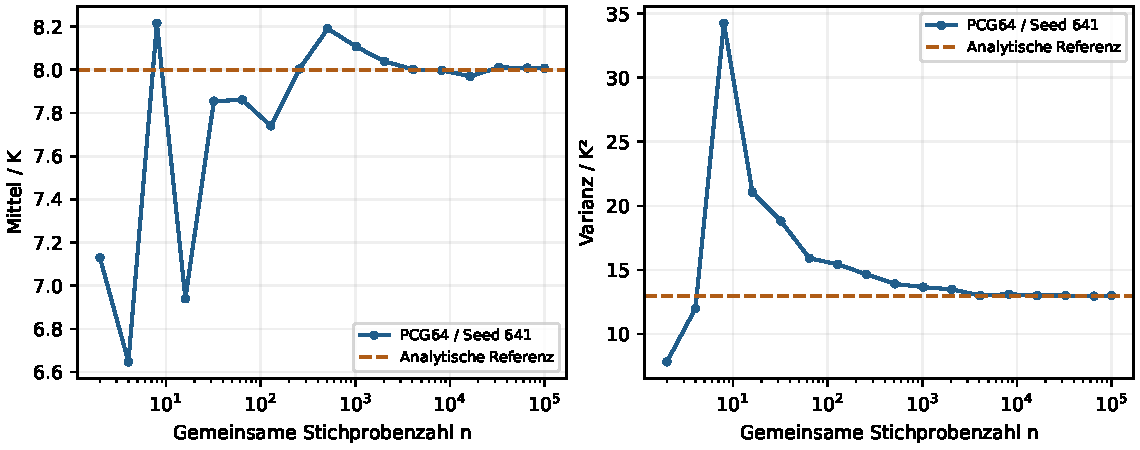
\includegraphics[width=\textwidth]{assets/verification-uncertainty.pdf}
\caption{Präfixschätzungen des synthetischen linearen Falls. Gestrichelte Linien
sind die unabhängig hergeleiteten Momente. Einzelne Präfixe können stärker
abweichen; die Darstellung behauptet keine monotone Konvergenz. Eigene Abbildung.}
\end{figure}

Der Ableitungsvergleich verwendet Schritte 0.01 und 0.02 sowie die analytisch
begründete Rundungsschranke $10^{-12}$ K. Die Ergebnisse und der Hash der
Little-Endian-float64-Samplebytes stehen in
\path{Doc/latex/evidence/uq-linear.json}. Die vollständigen Zeilen werden
aus Seed und Spezifikation reproduziert; sie sind nicht als Messbestand archiviert.

\section{Verifikation mit echten FEM-Aufrufen}
Der zusätzliche synthetische Wärmefall löst 128 gemeinsame Parameterzeilen
mit Seed 64 über \texttt{UncertaintyStudy}. Für die exakt diskret darstellbare
Zielgröße gilt $T_{\max}=T_0+Q/8$, mit
$Q\sim\mathcal U(4,12)$ W/m$^3$ und $T_0\sim\mathcal N(300,1)$ K
bei den im Rezept festgelegten Einheitsmaßen und Leitfähigkeit.
Damit folgen $\mathbb E[T_{\max}]=301$ K und
$\operatorname{Var}(T_{\max})=13/12$ K$^2$.
Der FEM-Vergleich jeder Zeile verwendet $10^{-11}$ K, der lokale
Gradientenvergleich mit $(1/8,1)$ die vorgegebene SI-Toleranz $2\cdot10^{-10}$.
Die kontinuierliche Diskretisierungsfehlerschranke ist weiterhin unbekannt,
also \texttt{None}. Der Fall ist keine Wärme- oder Piezomessung.

\section{Fehlerbudget und Fehlerstatus}
\index{Fehlerbudget}
Ein deterministischer numerischer Fehlerbetrag besitzt die Zieleinheit, eine
Varianz deren Quadrat. Sie werden nicht automatisch addiert. Im algebraischen
Lehrfall wird 0.01 K als \emph{illustrativer Nutzerbetrag} weitergereicht:
Er ist keine aus FEM-Konvergenz hergeleitete Schranke. Ein unbekanntes Budget
bleibt \texttt{None}; fehlende Kenntnis darf nicht durch Null ersetzt werden.

Für einen konkreten Verwendungszweck müssen Raumfehler, Zeitfehler,
algebraischer Fehler, Monte-Carlo-Schätzfehler, Eingabeunsicherheit,
Messunsicherheit und Modellabweichung getrennt begründet werden.
Eine spätere gemeinsame Rechnung benötigt passende probabilistische Annahmen
und Kovarianzen. Eine deterministische obere Schranke ist nicht ohne weitere
Annahmen eine Standardabweichung.

Jede gemeinsame Parameterzeile ist eine M8-Studie mit Modell-, Parameter-
und Tabellenvertrag. Bei irgendeinem fehlgeschlagenen Stichprobenfall werden
keine Teilmengenmomente ausgegeben; ein stiller Ausschluss könnte die Verteilung
verzerren. Ein Fehler nur in den zusätzlichen Sensitivitätsläufen unterdrückt
deren Gradient, ohne erfolgreiche Monte-Carlo-Werte umzudeuten.
Wiederaufnahme prüft Provenienz und Zielvertrag. Sperre und atomarer Report
verhindern konkurrierende oder teilweise geschriebene Erfolgsmeldungen.
